\chapter{Fungsi Pada Python}
\par Pada pembuatan program yang kompleks dan memiliki banyak fitur, kita diharuskan menggunakan fungsi. hal tersebut karena bisa jadi kita akan kerepotan menulis kode programnya, karena banyak yang harus ditulis dan kode akan menjadi sulit dibaca dan dirawat (maintenance).
\par Dengan fungsi, kita dapat memecah program besar menjadi sub program yang lebih sederhana. Masing-masing fitur pada program dapat kita buat dalam satu fungsi. Pada saat kita membutuhkan fitur tersebut, kita tinggal panggil fungsinya saja.Hal ini akan kita coba pada contoh program yang sudah saya sediakan di bawah.Namun, terlebih dahulu. Kita harus memahami teori dasar dan hal apa saja yang harus kita ketahui tentang fungsi di Python.
\section{Cara Membuat Fungsi Python}
Fungsi pada Python, dibuat dengan kata kunci def kemudian diikuti dengan nama fungsinya.

Contoh: \begin{lstlisting}
def nama_fungsi():
    print "Hello ini Fungsi"
\end{lstlisting}
 Sama seperti blok kode yang lain, kita juga harus memberikan identasi (tab atau spasi 2x) untuk menuliskan isi fungsi.
\newpage \begin{figure}[!htbp]
    \centering
    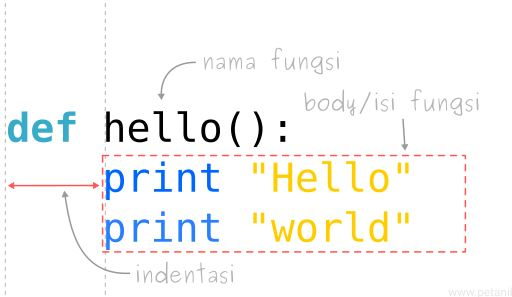
\includegraphics[scale=0.5]{figures/p2}
    \label{fungsi}
\end{figure}
\par Setelah kita buat, kita bisa memanggilnya seperti ini:
\begin{lstlisting}
nama_fungsi()
\end{lstlisting}
Sebagai contoh, coba tulis kode program berikut:
\begin{lstlisting}
# Membuat Fungsi
def salam():
    print "Hello World"

## Pemanggilan Fungsi
salam()
salam()
salam()
\end{lstlisting}
Hasilnya:
\begin{lstlisting}
Hello World
Hello World
Hello World
\end{lstlisting}
Intinya adalah apapun yang ada di dalam fungsi, ketika dipanggil itulah yang akan dilakukan.
\par FYI: fungsi juga dapat dipanggil pada fungsi lain, bahkan bisa memanggil dirinya sendiri. Fungsi yang memanggil dirinya sendiri, disebut fungsi rekursif.
\section{Fungsi Dengan Parameter}
\par Fungsi parameter merupakan variabel yang menampung nilai untuk diproses di dalam fungsi.
\par \textbf{Contoh}:
\begin{lstlisting}
def salam(ucapan):
    print(ucapan)
\end{lstlisting}
Pada contoh diatas, kita membuat fungsi dengan parameter ucapan.Kemudian cara untuk pemanggilan fungsi yang memiliki parameter tersebut adalah seperti berikut:
\begin{lstlisting}
salam("Selamat siang")
\end{lstlisting}
"Selamat siang" adalah nilai parameter yang kita berikan.
\par Untuk parameter yang lebih dari satu kita bisa menggunakan tanda koma (,) untuk memisahnya.
\par\textbf{Contoh}:
\begin{lstlisting}
# Membuat fungsi dengan parameter
def luas_segitiga(alas, tinggi):
    luas = (alas * tinggi) / 2
    print "Luas segitiga: %f" % luas;

# Pemanggilan fungsi
luas_segitiga(4, 6)
\end{lstlisting}
\par\textbf{Hasilnya}:
\begin{lstlisting}
Luas segitiga: 12.000000
\end{lstlisting}
\section{Fungsi Yang Mengembalikan Nilai}
Fungsi yang tidak mengembalikan nilai biasanya disebut dengan prosedur.
Tetapi, suatu waktu kita butuh hasil proses dari fungsi untuk digunakan pada proses berikutnya.Maka fungsi harus mengembalikan nilai dari hasil pemrosesannya.Cara mengembalikan nilai adalah menggunakan kata kunci \textit{return} lalu diikuti dengan nilai atau \textit{variabel} yang akan dikembalikan.
\par\textbf{Contoh}:
\begin{lstlisting}
def luas_persegi(sisi):
    luas = sisi * sisi
    return luas

# pemanggilan fungsi
print "Luas persegi: %d" % luas_persegi(6)
\end{lstlisting}
\par \textbf{Hasilnya}:
\begin{lstlisting}
Luas persegi: 36
\end{lstlisting}
Perbedaan dengan fungsi luas segitiga() yang sebelumnya adalah pada fungsi luas segitiga() kita melakukan print dari hasil pemrosesan secara langsung di dalam fungsinya. Sedangkan fungsi luas persegi(), kita melakukan print pada saat pemanggilannya.Jadi, fungsi luas persegi() akan bernilai sesuai dengan hasil yang dikembalikan.
Sehingga kita dapat memanfaatkannya untuk pemerosesan berikutnya.
\par\textbf{Seperti pada contoh berikut}:
\begin{lstlisting}
# rumus: sisi x sisi
def luas_persegi(sisi):
    luas = sisi * sisi
    return luas


# rumus: sisi x sisi x sisi
def volume_persegi(sisi):
    volume = luas_persegi(sisi) * sisi
\end{lstlisting}
\par Pada contoh di atas, kita melakukan pemanggilan fungsi luas persegi() untuk menghitung volume persegi.
\section{Variabel Global dan Lokal pada Python}
\par Variabel Global(berbeda file) adalah variabel yang bisa diakses dari semua fungsi, sedangkan variabel lokal(satu file) hanya bisa diakses di dalam fungsi tempat ia berada saja.Pada Python, urutan pengaksesan variabel (scope) dikenal dengan sebutan LGB (Local, Global, dan Build-in).Jadi program python mulai mencari vairabel lokal terlebih dahulu, kalau ada maka itu yang digunakan.Tetapi kalau tidak ada, pencarian terus ke Global, dan Build-in. Variabel Build-in adalah variabel yang sudah ada di dalam Python.
\par\textbf{Contoh program}:
\begin{lstlisting}
# membuat variabel global
nama = "Petanikode"
versi = "1.0.0"

def help():
    # ini variabel lokal
    nama = "Programku"
    versi = "1.0.2"
    # mengakses variabel lokal
    print "Nama: %s" % nama
    print "Versi: %s" % versi


# mengakses variabel global
print "Nama: %s" % nama
print "Versi: %s" % versi

# memanggil fungsi help()
help()
\end{lstlisting}
\par \textbf{Hasilnya}:
\begin{lstlisting}
Nama: Petanikode
Versi: 1.0.0
Nama: Programku
Versi: 1.0.2
\end{lstlisting}
\newpage Perhatikanlah variabel nama yang berada di dalam fungsi help() dan diluar fungsi `help(). Variabel nama yang berada di dalam fungsi help() adalah variabel lokal. Jadi, saat kita memanggil fungsi help() maka nilai yang akan tampil adalah nilai yang ada di dalam fungsi help(). Mengapa yang tampil tidak global di karenakan Python mulai mencari dari lokal, ke global, dan build-in. Jika di tiga tempat itu tidak ditemukan, maka biasanya akan terjadi NameError atau variabel tidak ditemukan.

\section{Contoh Program Dengan fungsi}
Berikut adalah langkah membuat program nya. Silahkan buat file baru bernama programfungsi.py. Lalu kita mulai tulis kodenya. Pertama kita buat sebuah variabel global berupa list untuk menampung judul-judul buku.
\begin{lstlisting}
# Variabel global untuk menyimpan data Buku
buku = []
\end{lstlisting}
Kemudian program ini akan mampu melakukan operasi CRUD (Create, Read, Update, dan Delete). Maka kita membutuhkan fungsi-fungsi berikut:
\begin{enumerate}
    \item show\_data() untuk menampilkan data dari list buku;
    \item insert\_data() untuk menambahkan data ke list buku;
    \item edit\_data() untuk mengedit data di list buku;
    \item delete\_data() untuk untuk menghapus data dari list buku.
\end{enumerate}
\par \textbf{Langkah Berikutnya adalah dimulai dari fungsi show\_data()}:
\begin{lstlisting}
# fungsi untuk menampilkan semua data
def show_data():
    if len(buku) <= 0:
        print "BELUM ADA DATA"
    else:
        for indeks in range(len(buku)):
            print "[%d] %s" % (indeks, buku[indeks])
            
\end{lstlisting}
Fungsi di atas akan mengecek isi dari list buku. Jika isinya kosong (len(buku) <= 0) maka tampilkan "BELUM ADA DATA". Namun, apabila ada isinya, maka tampilkan semua isinya dengan perulangan.
\par\textbf{Selanjutnya membuat fungsi insert\_data()}:
\begin{lstlisting}
# fungsi untuk menambah data
def insert_data():
    buku_baru = raw_input("Judul Buku: ")
    buku.append(buku_baru)
            
\end{lstlisting}
\par\textbf{Selanjutnya membuat fungsi edit\_data()}:
\begin{lstlisting}
# fungsi untuk edit data
def edit_data():
    show_data()
    indeks = input("Inputkan ID buku: ")
    if(indeks > len(buku)):
        print "ID salah"
    else:
        judul_baru = raw_input("Judul baru: ")
        buku[indeks] = judul_baru
\end{lstlisting}
Fungsi di atas akan menampilkan isi dari list buku dengan memanggil fungsi show\_data() di dalamnya. Setelah itu, kita meminta user untuk menginputkan ID atau nomer indeks buku yang akan diedit. Lalu kita lakukan pengecekan, jika ID yang diinputkan melebihi dari isi list buku (indeks > len(buku)), maka tampilkan pesan "ID salah". Namun, apabila tidak melebihi dari isi buku, maka ambil input untuk judul baru dan simpan sesuai ID-nya.
\par \textbf{Selanjutnya membuat fungsi delete\_data()}:
\begin{lstlisting}
# fungsi untuk menhapus data
def delete_data():
    show_data()
    indeks = input("Inputkan ID buku: ")
    if(indeks > len(buku)):
        print "ID salah"
    else:
        buku.remove(buku[indeks])
\end{lstlisting}
Hampir sama dengan fungsi edit\_data(). Fungsi delete\_data() juga harus menampilkan isi list buku dan mengambil ID yang akan dihapus. Kita dapat menghapus item pada list dengan fungsi remove().
 \par Setelah langkah di atas, ada 2 fungsi lagi yang di butuhkan:
 \begin{enumerate}
     \item Fungsi untuk menampilkan menu
     \item Fungsi untuk keluar (sudah ada di python: exit())
 \end{enumerate}
 \begin{lstlisting}
# fungsi untuk menampilkan menu
def show_menu():
    print "\n"
    print "----------- MENU ----------"
    print "[1] Show Data"
    print "[2] Insert Data"
    print "[3] Edit Data"
    print "[4] Delete Data"
    print "[5] Exit"
    
    menu = input("PILIH MENU> ")
    print "\n"

    if menu == 1:
        show_data()
    elif menu == 2:
        insert_data()
    elif menu == 3:
        edit_data()
    elif menu == 4:
        delete_data()
    elif menu == 5:
        exit()
    else:
        print "Salah pilih!"
\end{lstlisting}
Fungsi di atas akan menampilkan menu dari 1–5, lalu memanggil fungsi-fungsi yang sudah dibuat berdasarkan menu yang dipilih.

Terakhir, kita harus membuat main loop programnya.
\begin{lstlisting}
if __name__ == "__main__":
   
    while(True):
        show_menu()
\end{lstlisting}
Program akan mengulang terus-menerus sampai fungsi exit() dieksekusi.

if \_\_name\_\_ == "\_\_main\_\_": adalah blok main di Python. Sebenarnya tanpa ini, programnya sudah bisa dijalankan namun agar lebih bagus kita baiknya menambahkannya.
\par\textbf{Sehingga kode lengkapnya akan seperti ini}:
\begin{lstlisting}
# Variabel global untuk menyimpan data Buku
buku = []


# fungsi untuk menampilkan semua data
def show_data():
    if len(buku) <= 0:
        print "BELUM ADA DATA"
    else:
        for indeks in range(len(buku)):
            print "[%d] %s" % (indeks, buku[indeks])


# fungsi untuk menambah data
def insert_data():
    buku_baru = raw_input("Judul Buku: ")
    buku.append(buku_baru)

# fungsi untuk edit data
def edit_data():
    show_data()
    indeks = input("Inputkan ID buku: ")
    if(indeks > len(buku)):
        print "ID salah"
    else:
        judul_baru = raw_input("Judul baru: ")
        buku[indeks] = judul_baru

# fungsi untuk menhapus data
def delete_data():
    show_data()
    indeks = input("Inputkan ID buku: ")
    if(indeks > len(buku)):
        print "ID salah"
    else:
        buku.remove(buku[indeks])

# fungsi untuk menampilkan menu
def show_menu():
    print "\n"
    print "----------- MENU ----------"
    print "[1] Show Data"
    print "[2] Insert Data"
    print "[3] Edit Data"
    print "[4] Delete Data"
    print "[5] Exit"
    
    menu = input("PILIH MENU> ")
    print "\n"

    if menu == 1:
        show_data()
    elif menu == 2:
        insert_data()
    elif menu == 3:
        edit_data()
    elif menu == 4:
        delete_data()
    elif menu == 5:
        exit()
    else:
        print "Salah pilih!"


if __name__ == "__main__":

    while(True):
        show_menu()
\end{lstlisting}
